\section*{}
The research purposes a solution based on deep convolutional neural networks
With various experiments mentioned in further sub-sections.  The experiments
require specific configuration for cuda libraries to run programs on available GPU(Graphical Processing Unit) for faster processing
and further, instructions to setup environment can be found at Tensorflow gpu installation guide \footnote[1]{\url{https://www.tensorflow.org/install/gpu}}.
Alternatively, the machine learning models can also run without installing cuda libraries on CPU but the processing will be slow.
In addition, the convolutional neural network was implemented using Python3 and Jupyter notebooks were used in these experiments which provides an appropriate interface to experiment and write markdowns.  
Jupyter notebooks can be installed by installing Anaconda \footnote[2]{https://www.anaconda.com/distribution/}.
Furthermore, data science and machine learning libraries are required such as Numpy, Keras, Matplotlib and OpenCV. 
Numpy library is required for performing mathematical operations on multi-dimensional NumPy arrays. The matplotlib library provides an interface to visualise the output results. 
The OpenCV library was used for image processing in the process of developing an automated system for classifying
pigmented skin lesions. Moreover, keras library was used to develop deep convolutional models. 
HAM,1000 (Human Against Machine, 1000) dataset was used to develop image classifier \citep{DVN/DBW86T_2018}.
The dataset primarily contains two folders which includes overall 10,000 dermatoscopic images of pigmented skin lesion. In addition, it also contains a CSV file which includes the meta-information regarding pigmented skin lesions.
The required files can be downloaded from harvard dataverse webiste \footnote[3]{\url{https://dataverse.harvard.edu/dataset.xhtml?persistentId=doi:10.7910/DVN/DBW86T}}.

\pagebreak
\section{Data Processing and Normalisation}
\begin{figure} [!htp]
    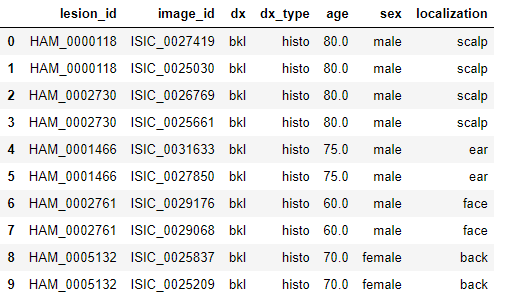
\includegraphics[width=\textwidth]{Images/datae.png}
    \caption{Pandas Dataframe containing information about pigmented skin lesions}
    \label{fig:pandasTop}
\end{figure}

The information was read using pandas into the data frame, 
which is a data structure that allows storing tabular data from CSV files as showm in 
figure \ref{fig:pandasTop}.The CSV file contained irrelevant information such as sex, age and localisation 
of patients in the data frame which was removed by dropping the non esential columns.
In addition, the dataset contains unclear and hairy images of pigmented skin lesions which were manually 
removed from the dataset to enhance the quality of available data.
Furthermore, the research only focuses on limited categories of 
pigmented skins which results in dropping data columns for the other categories 
of data. The information shown in above dataframe contains a lesionid column which coresponds
to image names which were were read into numpy array using pillow library from respective directories.
The data for convolutional neural networks needs to divided into training and testing data, the model learnings
are peformed with learning the patterns and relationships in the training datasets and evaluation of the 
model is performed on the testing data which is never feed to the intelligent model which training.
The dataset was divided into training and testing sets using \url{sklearn.model_selection.train_test_split} class in the portion of 80 per cent for 
the training dataset and 20 per cent of testing datasets. The next step towards to preparing the dataset was reading the images data into NumPy 
array for both training and testing datasets and converting the image names from pandas series to NumPy array corresponding to each image and assign class number 
based on category of pigmented skin lesion in the dataset. Furthermore, the training and testing datasets were serialised into 
dictionary in a pickle encoded file. Therefore, the encoded file sizes are compact and are portable
in comparison to storing actual image files.
\subsection{Data Normalisation}
The images with RGB(Red, Green and Blue) channels information was stored in numpy mutli-demensional array with numbers ranging from 0 to 255.
The numpy array was converted into the float32 format and each element of the array was divided by 255 to normalise the data so, that 
it only ranges between 0 and 1 in float format which will help while training the model. In addition, one hot encoding 
was performed on class labels of the pigmented lesions. The one hot encoding is a representation of categorical variable 
as binary vector and normalise the categorical labels into binary vector.
\subsection{ Image Segmentation }
\begin{center}
	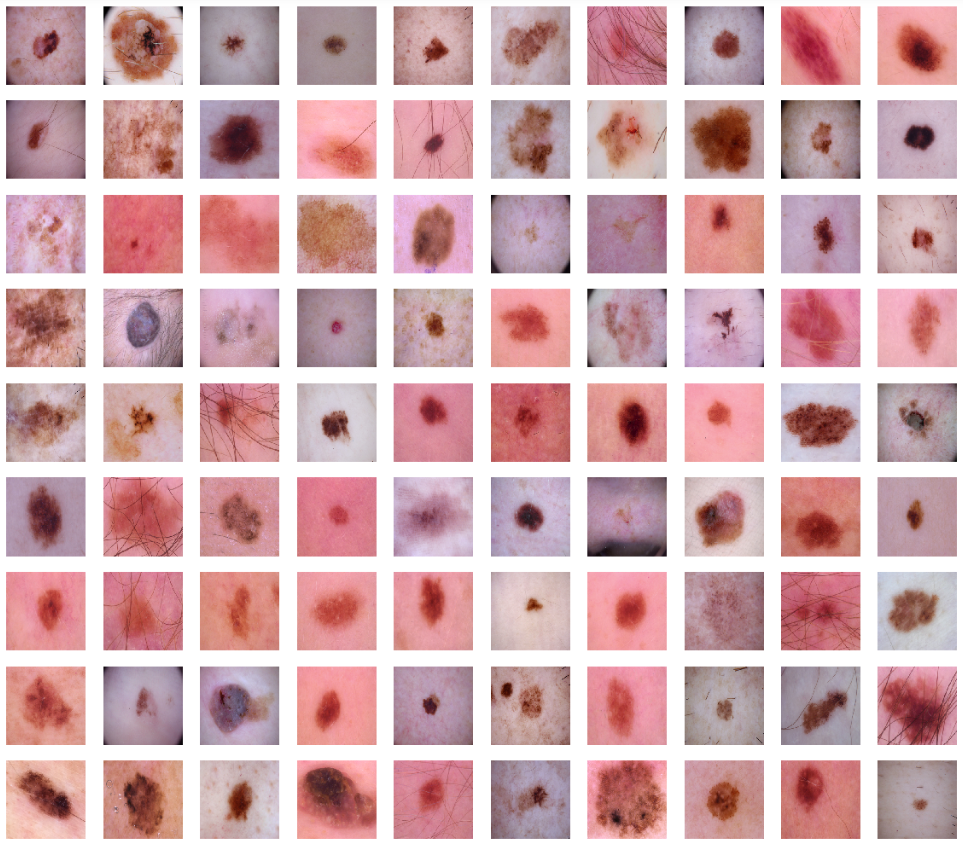
\includegraphics[width=10cm]{Images/bseg.png}
\end{center}

The figure above reflects the sample from training dataset before performing image segmentation.
The image segmentation was performed on the all the images using binary thresholding in OpenCV framework.

\section{Thresholding Segmentation Algorithm}

Thresholding is one of the commonly adopted method in image segmentation which helps in descrimination most 
significant pixels in the images \citep*{al2010image}. The thresold value is selected and the gray scale images  
are converted into the binary representation of the image and value of image which are greater than the thresold
value will be selected with keeping all the attributes of the images such as position and shape \citep*{al2010image}. 
Thus, reducing the complexity of the image data and making it easier for classification related tasks. Futhermore, the 
segmented images will be consumed in the model training. The thresholding segmentation was performed using OpenCV library using 
\url{cv.threshold(image, 0.5, 1, cv.THRESH_BINARY)} where threshold value of 0.5 and maximum value of the pixel can be 1
as it was normalised.

\begin{center}
	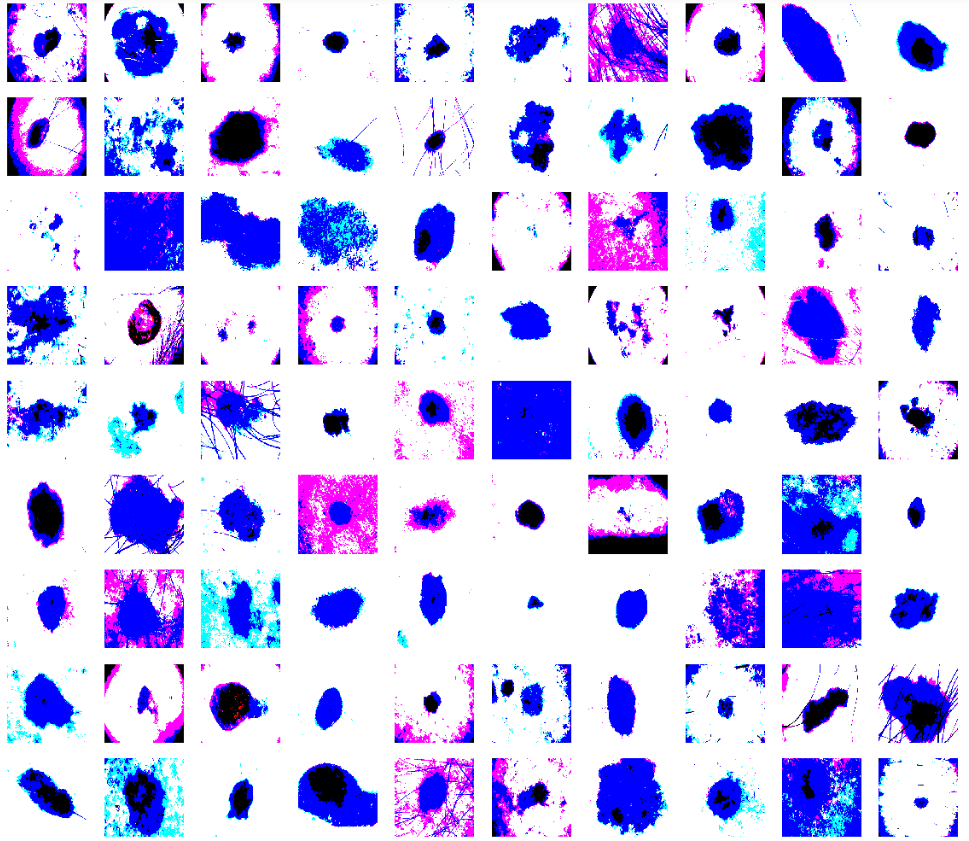
\includegraphics[width=10cm]{Images/aseg.png}
\end{center}

The figure above shows the result of applying the threshold image segmentation on pigmented skin lesions. 

\pagebreak
\section{Convolutional Model Training}

\begin{figure}
    \centering
    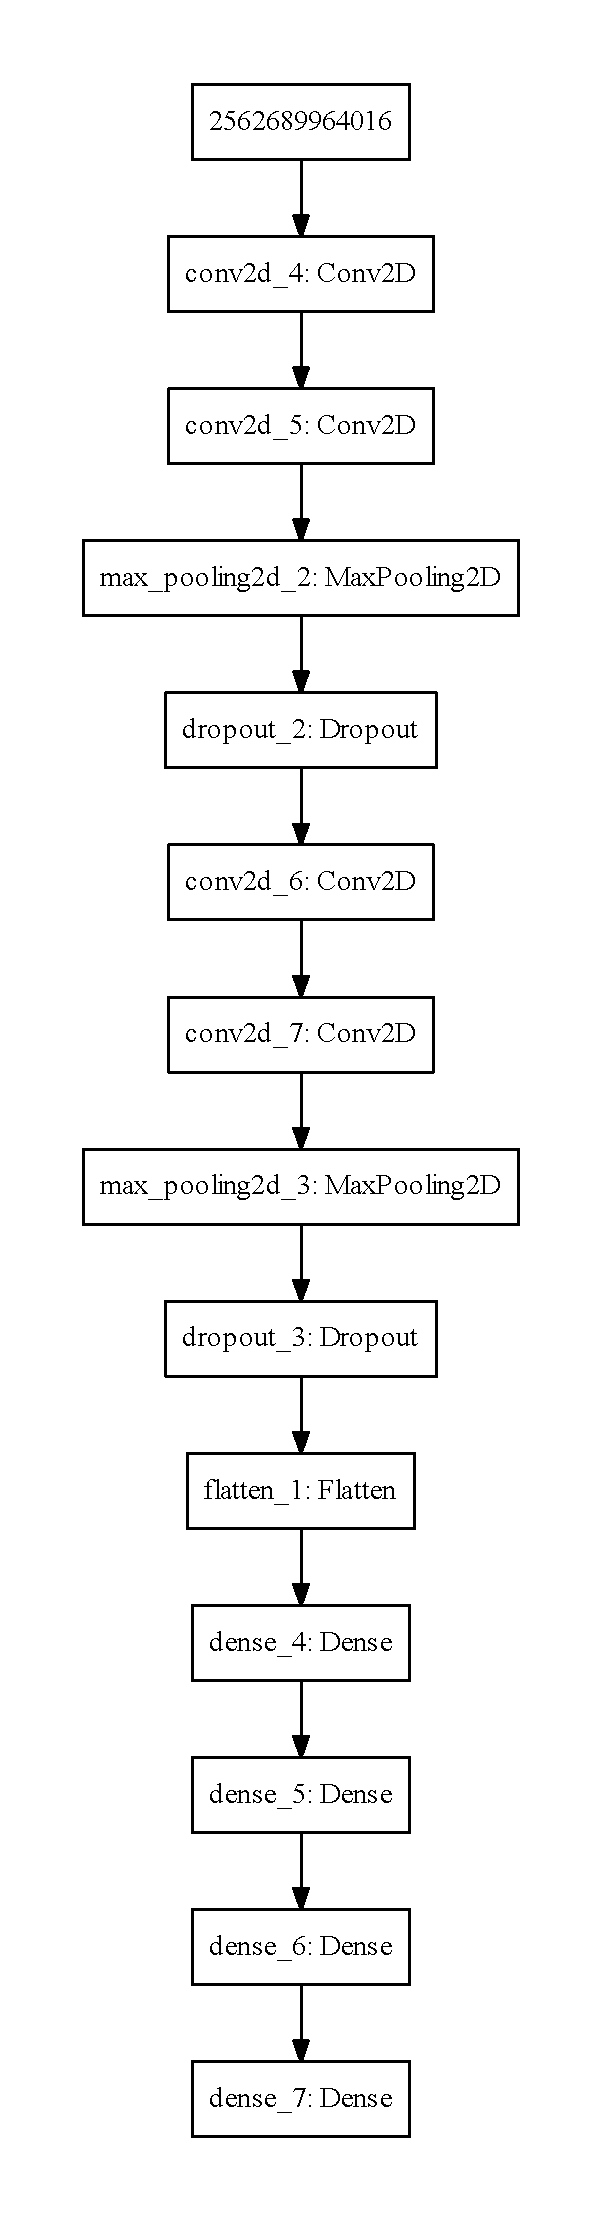
\includegraphics[height=.9\textheight]{Documents/model.pdf}
    \caption{Model Architecture 1}
\end{figure}
